\documentclass[tikz,border=16mm]{standalone}
\usepackage[normalem]{ulem}
\usetikzlibrary{positioning,fit,calc,backgrounds}
\tikzset{block/.style={draw,thick,text width=2cm,minimum height=1cm,align=center},
         line/.style={-latex}
}
\makeatletter
\def\ruwave{\bgroup \markoverwith{\lower7\p@\hbox{\textcolor{red}{\sixly \char116}}}\ULon}
\font\sixly=lasy6
\makeatother


\begin{document}
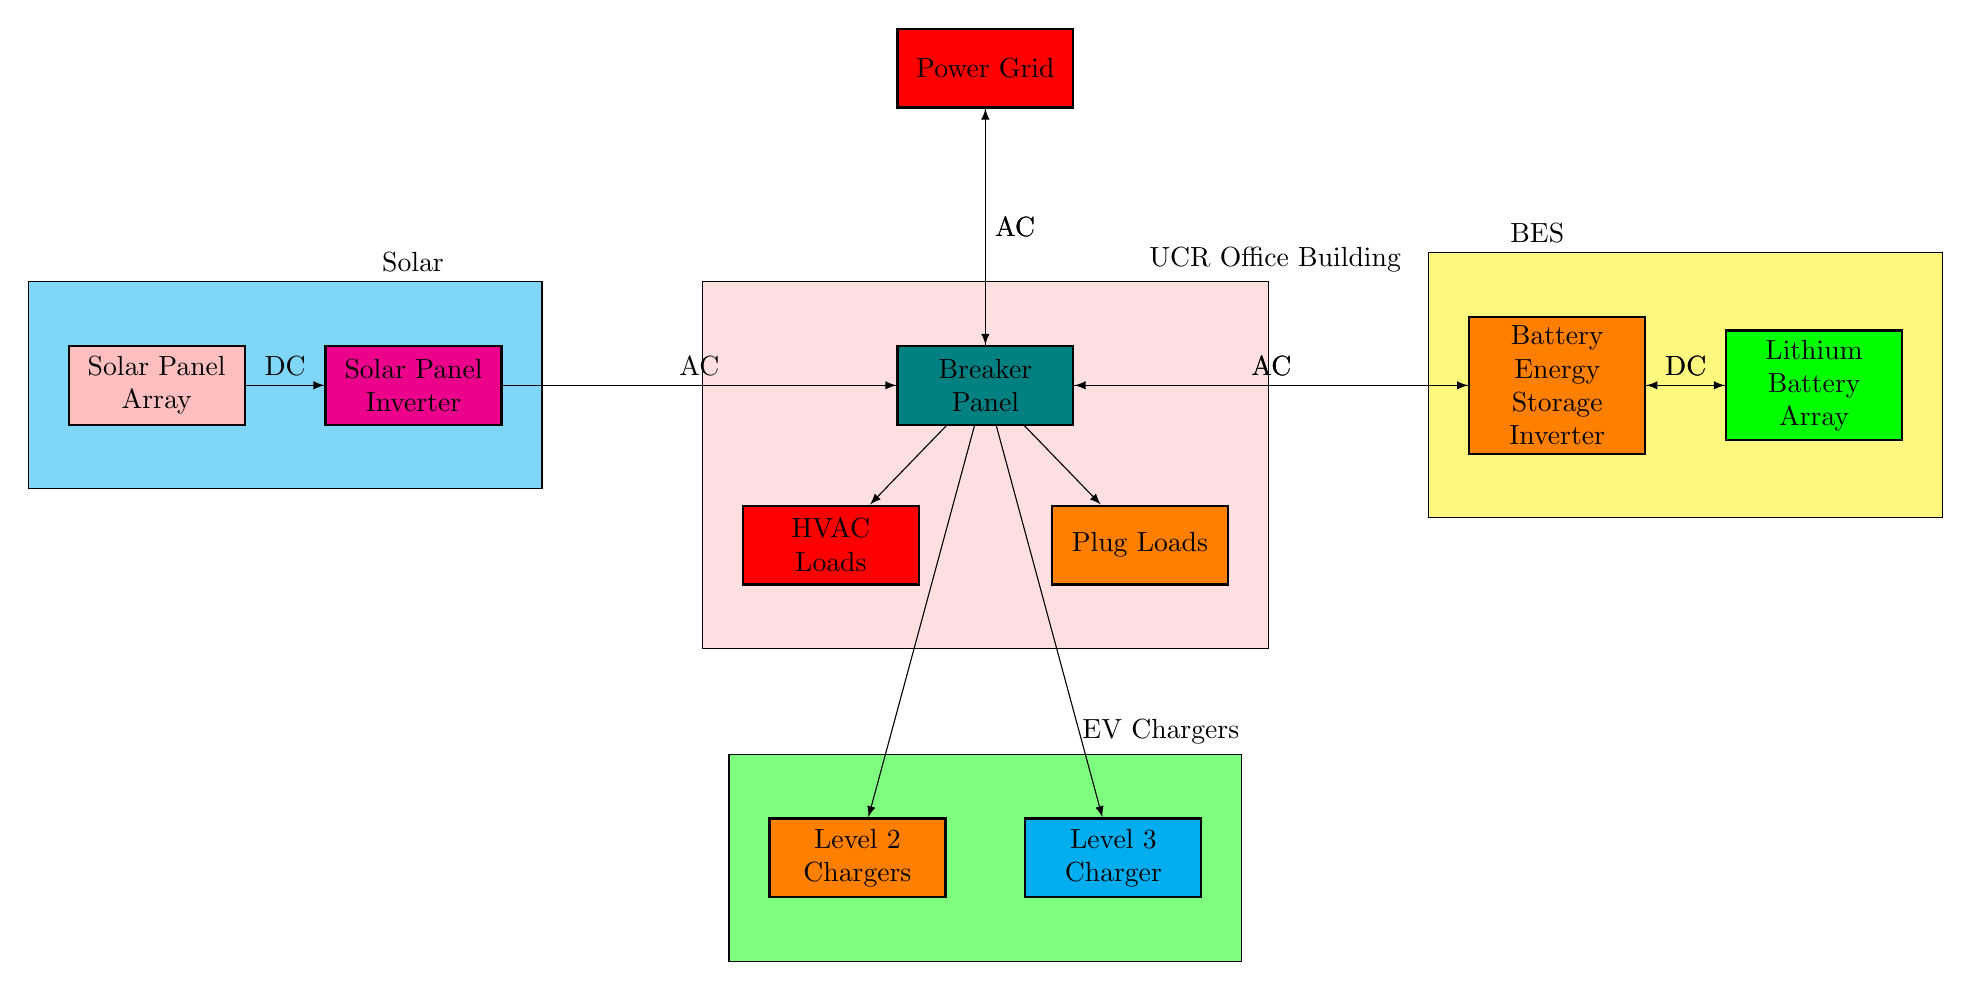
\begin{tikzpicture}
  \node[block, fill = teal] (a) at(0,0) {Breaker Panel};
  \node[block, fill = orange, right=of a, xshift = 4cm] (b) {Battery Energy Storage Inverter};
  \node[block, fill = green,right= of b] (c) {Lithium Battery Array};
  \node[block, fill = magenta, left=of a, xshift  = -4 cm] (d) {Solar Panel Inverter};
  \node[block, fill = pink, left=of d] (e) {Solar Panel Array};
  \node[block,fill = red, above =of a, yshift = 2cm] (q) {Power Grid};
  \node[block,fill = orange] (l) at (-1.625,-6) {Level 2 Chargers};
  \node[block,fill = cyan] (n) at (1.625,-6) {Level 3 Charger};
  \node[block,fill=red, below left =of a, xshift = 1.3cm] (o) {HVAC Loads};
  \node[block,fill = orange, below right= of a, xshift = -1.3cm] (j){Plug Loads};
%  \node[block,fill = orange, below of= e] (l)  {Level 2 Chargers};
%  \node[block,fill = cyan, below of= q] (n) at {V2G Charger};
  
  
  
  %\node[block] (e) at ([yshift=-2cm]$(b)!0.5!(c)$) {Gate};
  \begin{scope}[on background layer]
   %\node[draw,inner xsep=5mm,inner ysep=6mm,fit=(b)(c),fill=magenta!40]{};
   \node[draw,fill=yellow,fill opacity=0.5,inner xsep=5mm,inner
     ysep=8mm,fit=(b)(c),label={130:BES}](f){};
  \node[draw,fill=cyan,fill opacity=0.5,inner xsep=5mm,inner
     ysep=8mm,fit=(d)(e),label={50:Solar}]{};
  \node[draw,fill=green,fill opacity=0.5,inner xsep=5mm,inner
  	 ysep=8mm,fit=(l)(n),label={50:EV Chargers}]{};
  \node[draw,fill=pink,fill opacity=0.5,inner xsep=5mm,inner
	 ysep=8mm,fit=(a)(o)(j),label={50:UCR Office Building}]{};
  \end{scope}
  \draw[line] (q)-- (a) -- node [text width=2.5cm,midway,right,align=left] {AC} (q);
  \draw[line] (a)-- (q) -- node [text width=2.5cm,midway,right,align=left] {AC} (a);
  \draw[line] (b)-- (a) -- node [text width=2.5cm,midway,above,align=center] {AC} (b);
  \draw[line] (c) -- (b) -- node [text width=2.5cm,midway,above,align=center] {DC} (c);
  \draw[line] (a)-- (b) -- node [text width=2.5cm,midway,above,align=center] {AC} (a);
  \draw[line] (b) -- (c) -- node [text width=2.5cm,midway,above,align=center] {DC} (b);
  \draw[line] (a) -- (d) -- node [text width=2.5cm,midway,above,align=center] {AC} (a);
  \draw[line] (d) -- (e) -- node [text width=2.5cm,midway,above,align=center] {DC} (d);
  \draw[line] (a) -- (l) (l);
  \draw[line] (a) -- (n) (n);
  \draw[line] (a) -- (o) (o);
  \draw[line] (a) -- (j) (j);
%  \draw[line] (n) -- (a)  (a);
%  \draw[line] (a) -- (l) -- node [text width=1.0cm,midway,above,align=right] {AC} (l);
%  \draw[line] (a) -- (n) -- node [text width=1.0cm,midway,above,align=right] {AC} (n);
%  \draw[line] (n) -- (a) -- node [text width=1.0cm,midway,above,align=right] {AC} (a);
  
  
  
  %\draw[line] (f.east) -- (c)node[pos=0.4,above]{flow};
  %\draw[line] (e)-- ($(b)!0.5!(c)$);
\end{tikzpicture}
\end{document}